\chapter{Модель интеграции технологического ядра
  XiYan-SQL во внешний сервис}\label{chapter2}

\begin{annotation}
	В данной главе рассматривается современный, многокомпонентный подход к построению систем Text-to-SQL. Анализируется эволюция архитектур от монолитных моделей к системам, использующим инструменты и протоколы взаимодействия, такие как Model Context Protocol (MCP). Формулируется ключевая разработческая задача, заключающаяся в проектировании программного компонента-организатора для управления жизненным циклом запроса в такой сложной системе. Предлагается и детально описывается архитектурное решение этой задачи, которое ляжет в основу программной реализации в следующей главе.
\end{annotation}




\section{Рабочий процесс, предлагаемый XiYan-SQL}\label{sec:xiyan_workflow}

Фреймворк XiYan-SQL представляет собой инновационный подход к решению задач преобразования
естественного языка в SQL (Text-to-SQL), использующий ансамбль из нескольких
генераторов для улучшения качества и разнообразия кандидатов~\cite{gaoPreviewXiYanSQLMultiGenerator2025}.
Его рабочий процесс, который проиллюстрировать(см.~рис.~\ref{fig:xiyan-sql-workflow}),
можно разделить на три основных компонента: связывание со схемой, генерация кандидатов и
выбор итогового кандидата.

\begin{figure}[!htb]
	\centering
	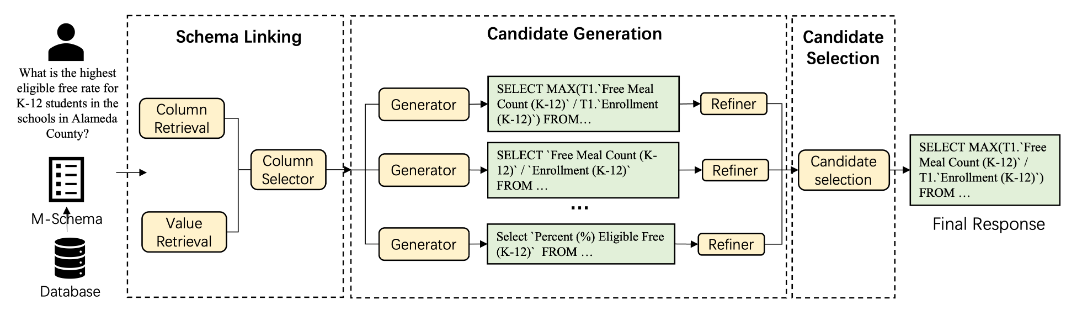
\includegraphics[width=1\textwidth]{literature-review/xiyan-sql-workflow.png}
	\caption{Схема рабочего процесса, предлагаемого XiYan-SQL}
	\label{fig:xiyan-sql-workflow}
\end{figure}


\paragraph{Связывание со схемой (Schema Linking)}. Это первый и ключевой этап, на котором
система анализирует запрос пользователя и обширную схему базы данных.
Его задача~--- отобрать только релевантные для запроса таблицы и столбцы,
а также извлечь из них необходимые значения. Это позволяет минимизировать количество
ненужной информации и сосредоточиться на данных, имеющих отношение к задаче.
Результат этого этапа представляется в виде компактной и четкой
полуструктурированной схемы \textit{M-Schema}, которая передается на следующий этап.

\paragraph{Генерация кандидатов (Candidate Generation)}. На этом этапе в работу вступают
несколько различных генераторов SQL-запросов. XiYan-SQL комбинирует два подхода:
\begin{compactitem}
	\item \textbf{Генераторы на основе Fine-Tuning (SFT)}. Специализированные модели,
	тонко настроенные на генерацию высокоточных и стилистически разнообразных SQL-запросов.
	\item \textbf{Генераторы на основе In-Context Learning (ICL)}. Используются для
	повышения гибкости и способности генерировать сложные запросы,
	используя возможности больших языковых моделей (LLM) с помощью тщательно подобранных примеров.
\end{compactitem}
Каждый сгенерированный кандидат затем проходит через модуль \textit{Refiner},
который пытается исправить возможные логические или синтаксические ошибки,
используя результаты выполнения запроса или информацию об ошибках.

\paragraph{Выбор кандидата (Candidate Selection)}. После получения набора разнообразных и
исправленных SQL-кандидатов, финальный компонент определяет наилучший вариант.
Вместо простого выбора самого частого запроса (self-consistency),
XiYan-SQL использует специально обученную модель, которая оценивает все нюансы кандидатов в
контексте исходного вопроса и схемы данных, чтобы выбрать наиболее корректный и разумный SQL-запрос.

Такая многокомпонентная архитектура позволяет XiYan-SQL достигать высокой точности и надежности в решении сложных задач Text-to-SQL в различных сценариях \cite{gaoPreviewXiYanSQLMultiGenerator2025}.




\section{Эволюция интеграции LLM с внешними программами}

Как было показано в предыдущей главе, большие языковые модели (LLM) стали технологическим ядром
современных NLIDB. Анализ показывает, что за последние годы произошла стремительная эволюция подходов
к интеграции LLM с внешними инструментами и сервисами, которую можно условно разделить на три этапа
(см.~рис.~\ref{fig:llm-evolution}).

\begin{figure}[h!]
	\centering
	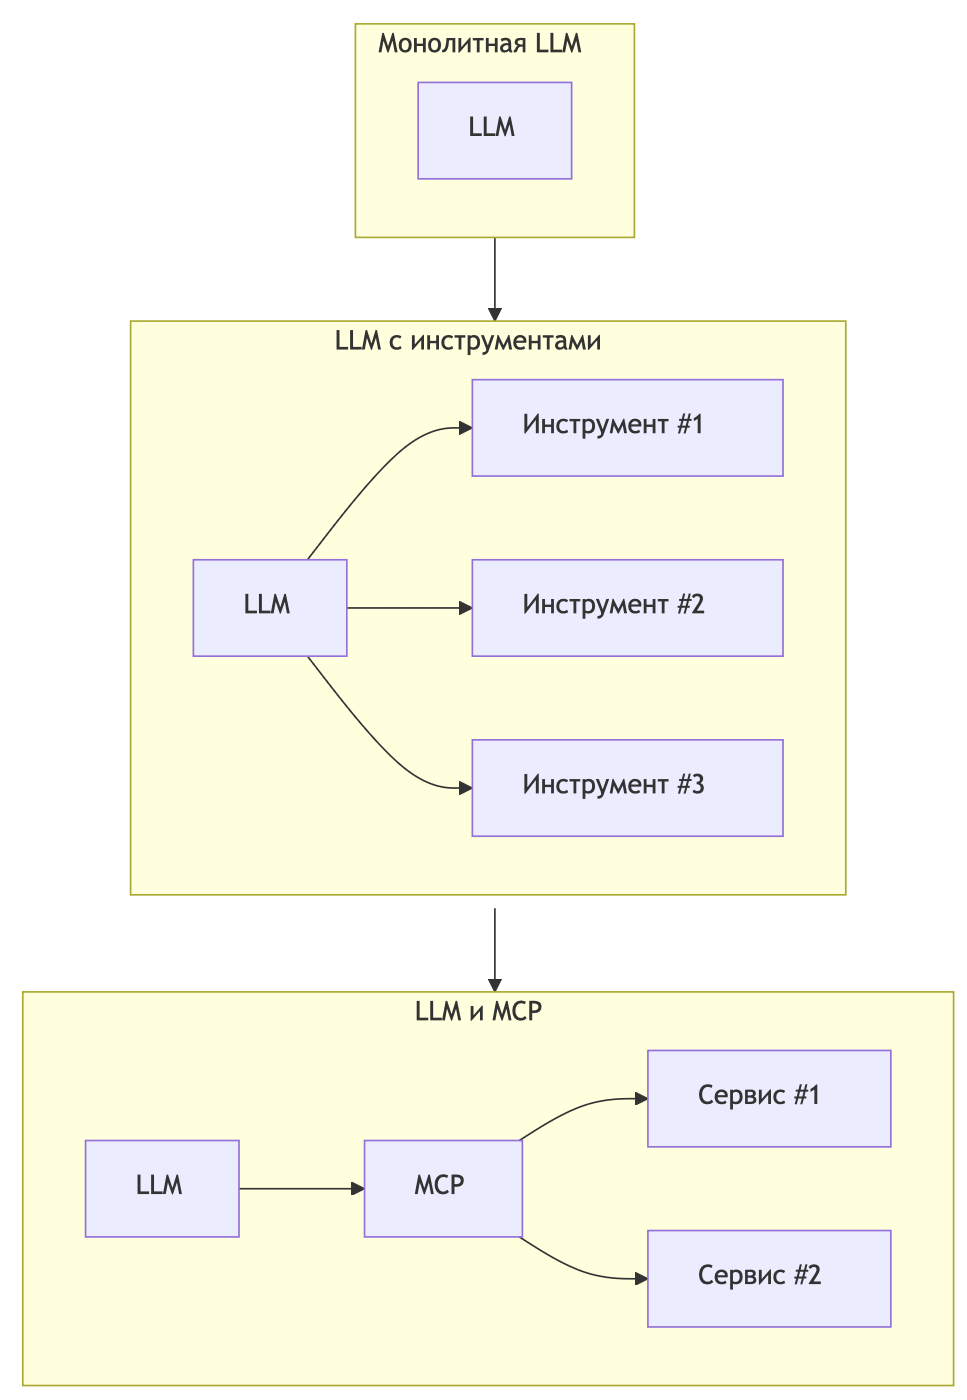
\includegraphics[width=1\textwidth]{created-diagrams/llm-evolution.png}
	\caption{Три этапа эволюции внедрения LLM-систем во внешние сервисы}
	\label{fig:llm-evolution}
\end{figure}

\paragraph{Этап I: Монолитная LLM}. На начальном этапе LLM использовалась как целостный «черный ящик».
Весь контекст, включая вопрос пользователя и полную схему базы данных,
передавался в модель одним запросом, а на выходе ожидался, если смотреть в контексте задачи Text-to-SQL,
готовый SQL-код.
Этот подход прост в реализации, но страдает от ряда фундаментальных проблем: неспособность
эффективно работать в контексте задачи, отсутствие контроля над процессом генерации и
сложность в отладке.

\paragraph{Этап II: LLM с инструментами}. Следующим шагом стало наделение LLM возможностью
использовать внешние инструменты через вызовы API. Например, модель могла сначала
вызвать инструмент для поиска по веб-страницам, а затем использовать полученную информацию
для ответа. Этот подход значительно расширил возможности LLM. Однако он породил новую
проблему, вызванную отсутствием стандарта. Каждый инструмент и сервис имеет собственный,
уникальный способ вызова и формат данных, что приводит к необходимости писать большое
количество связующего кода и усложняет масштабирование системы при добавлении
новых инструментов.

\paragraph{Этап III: LLM и стандартизированные протоколы (MCP)}. В конце
2024 года появился стандарт~--- \textit{Model Context Protocol (MCP)}.
MCP~--- это открытый протокол,
который стандартизирует способ, которым LLM (или AI-агенты) взаимодействуют с внешними инструментами и
источниками данных. Он действует как универсальное связующее звено между моделью и
сервисами, позволяя им общаться на едином, стандартизированном языке. Это решает проблему
масштабируемости и значительно упрощает добавление новых инструментов в экосистему.

Фреймворк XiYan-SQL, выбранный в качестве технологического ядра для данного проекта,
предоставляет реализацию такого подхода в виде \textit{XiYan-SQL MCP
	Server} \footnote{URL: \url{https://github.com/XGenerationLab/xiyan_mcp_server}}.
Этот сервер является не единой моделью, а ансамблем из нескольких независимых модулей,
взаимодействие с которыми происходит по протоколу MCP. Такая архитектура является передовой,
однако она порождает новую, нетривиальную разработческую задачу.




\section{Протокол MCP (Model Context Protocol)}

\textit{Model Context Protocol (MCP)}~---
открытый, стандартизированный протокол, призванный стать универсальным языком для
общения между AI-модулями и внешними источниками данных или инструментами.

MCP действует как универсальное связующее звено,
которое стандартизирует способ, которым AI-модуль запрашивает информацию или действие у
инструмента и получает ответ. Протокол определяет четкую и единую структуру для сообщений,
которыми обмениваются компоненты системы. Таким образом, вместо того чтобы напрямую
обращаться к уникальному API каждого инструмента, модул формирует стандартизированный
MCP-запрос. Специальный адаптер на стороне инструмента преобразует этот запрос в вызов
своего API и возвращает ответ также в стандартном MCP-формате.

К примеру, XiYan MCP Server
предлагает архитектуру, позволяющую два способа интегрировать сервер в проект: локальный и
удаленный (см.~рис.~\ref{xiyan-mcp-server-architecture}).

\begin{figure}
	\begin{center}
		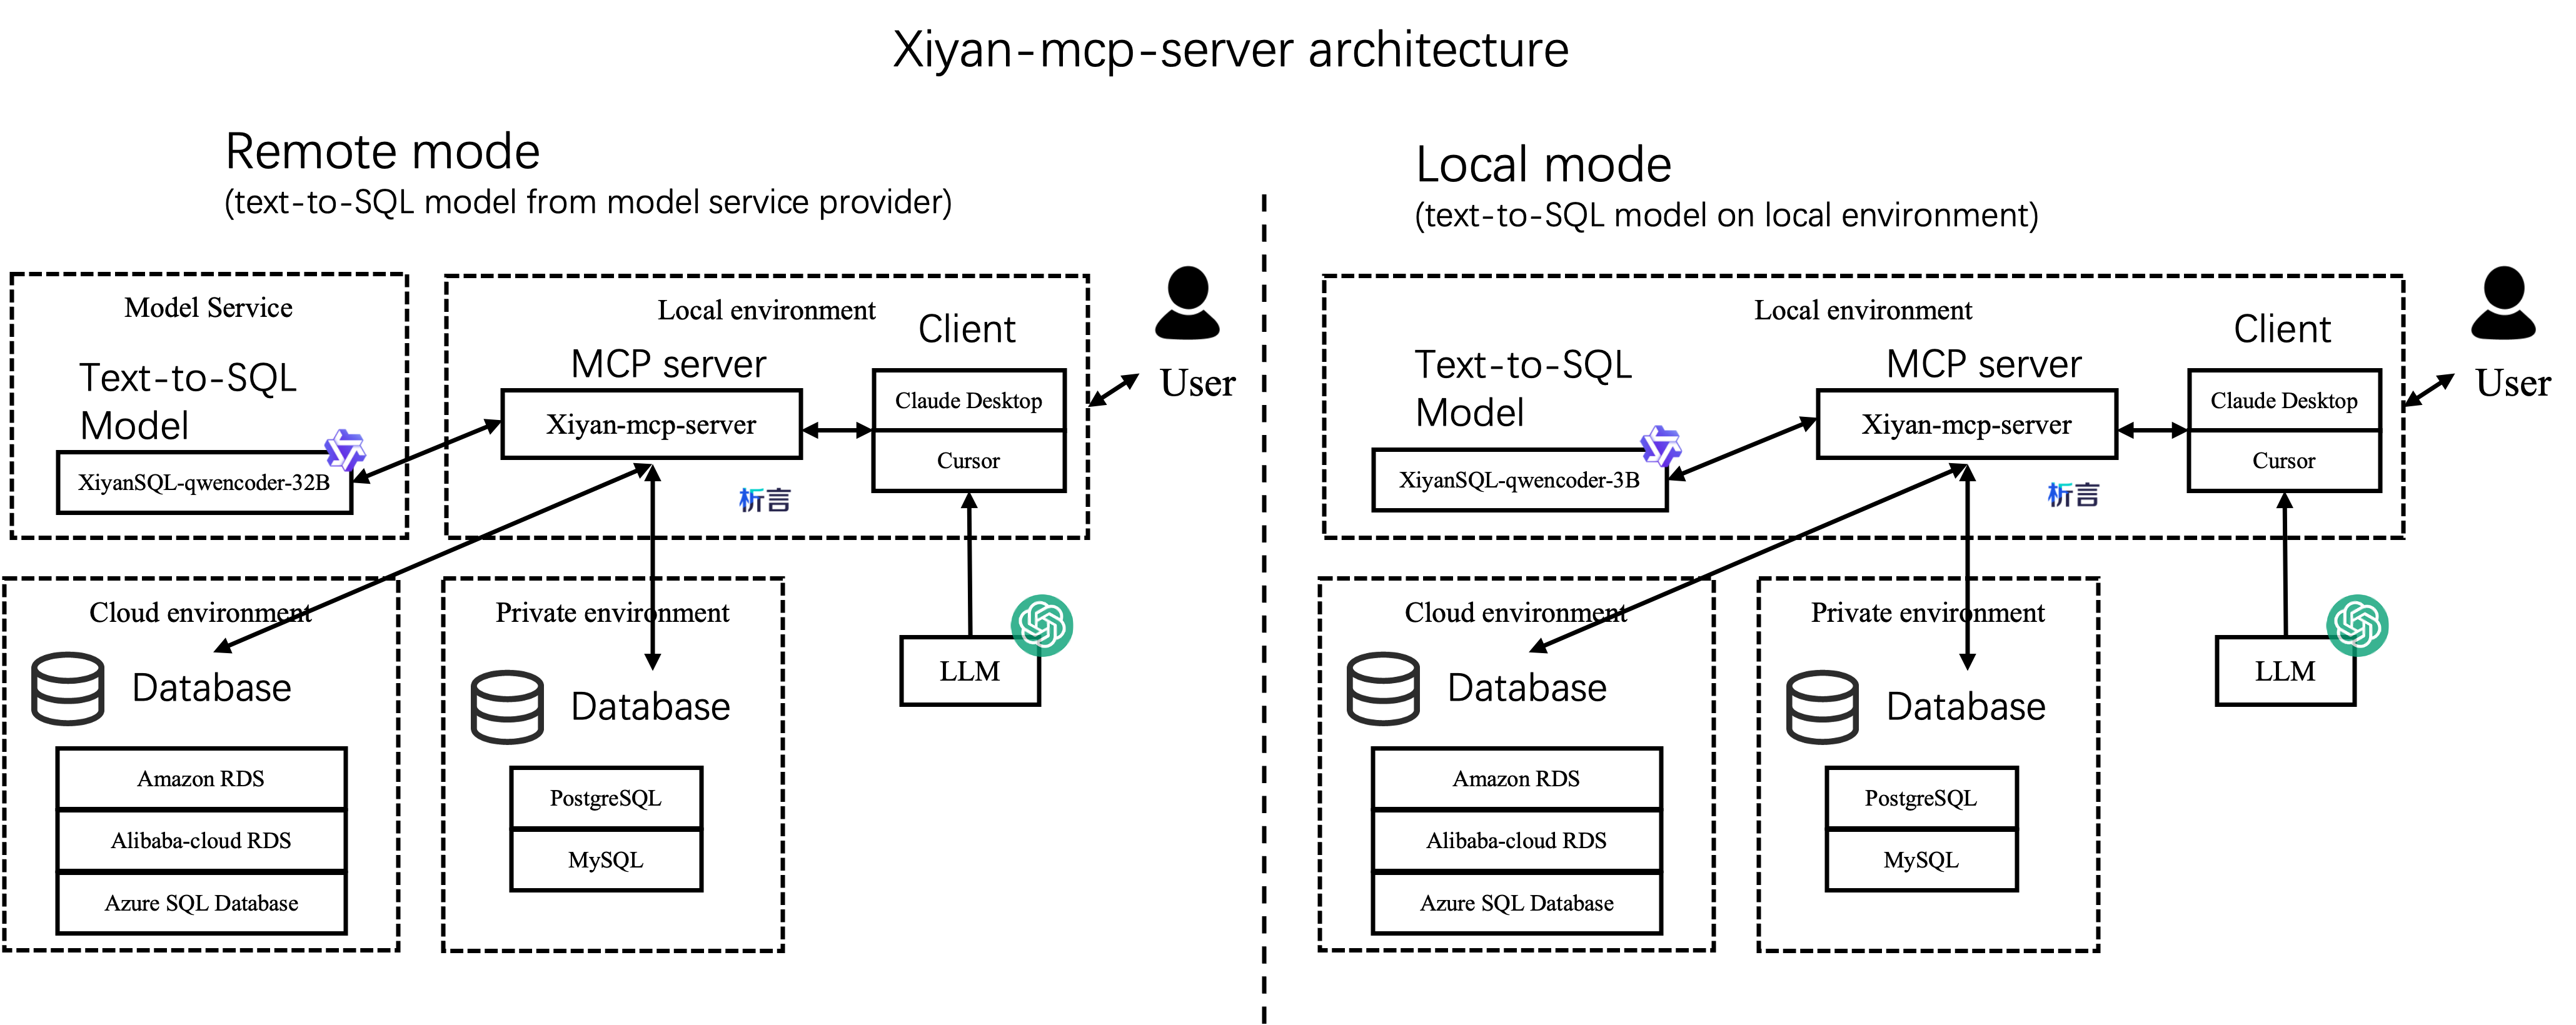
\includegraphics[width=1\textwidth]{literature-review/xiyan-mcp-server-architecture.png}
	\end{center}
	\caption{Архитектура технологического ядра XiYan MCP Server}
	\label{xiyan-mcp-server-architecture}
\end{figure}

Внедрение MCP в архитектуру AI-систем дает несколько значительных преимуществ: модульность и
взаимозаменяемость инструментов и моделей, масштабируемость системы и простота разработки.
Несмотря на преимущества, у протокола есть и текущие ограничения. Во-первых,
как дополнительный уровень абстракции, он может вносить небольшую задержку
в выполнение запросов. Во-вторых, будучи новым стандартом, он может пока не покрывать
все специфические случаи использования для каждого возможного инструмента.
Примеры применения включают:
\begin{compactitem}
	\item AI-ассистентов, использующих внешние сервисы (заказ билетов, прогноз погоды).
	\item Корпоративные чат-боты, подключенные к внутренним базам знаний.
	\item Сложные системы, где несколько специализированных AI-модулей совместно решают задачу,
	обмениваясь данными через MCP.
\end{compactitem}
\noindent Перспективы MCP связаны с формированием
глобального «рынка» совместимых AI-инструментов. Это стимулирует появление специализированных
сервисов-«оркестраторов», управляющих сложными цепочками вызовов между модулями.




\section{Моделирование MCP-клиента для интеграции с ядром XiYan-SQL}

Как было установлено, технологическое ядро XiYan-SQL представляет собой \textit{MCP-сервер},
который предоставляет доступ к ансамблю независимых AI-модулей. Для интеграции такого ядра во
внешний веб-сервис необходимо спроектировать на стороне сервиса соответствующий \textbf{MCP-клиент}.
Этот компонент будет отвечать за всю логику взаимодействия с ядром,
выступая в роли «Организатора» или «Оркестратора» полного жизненного цикла обработки
пользовательского запроса.

Задача данного компонента~--- инкапсулировать сложную, многошаговую последовательность
вызовов к различным модулям MCP-сервера, предоставляя остальной части веб-приложения
простой и высокоуровневый интерфейс. Цикл обработки одного запроса, управляемый MCP-клиентом,
состоит из нескольких последовательных шагов, как показано на схеме
(см.~рис.~\ref{fig:mcp-client-flow}).

\begin{figure}[ht]
	\centering
	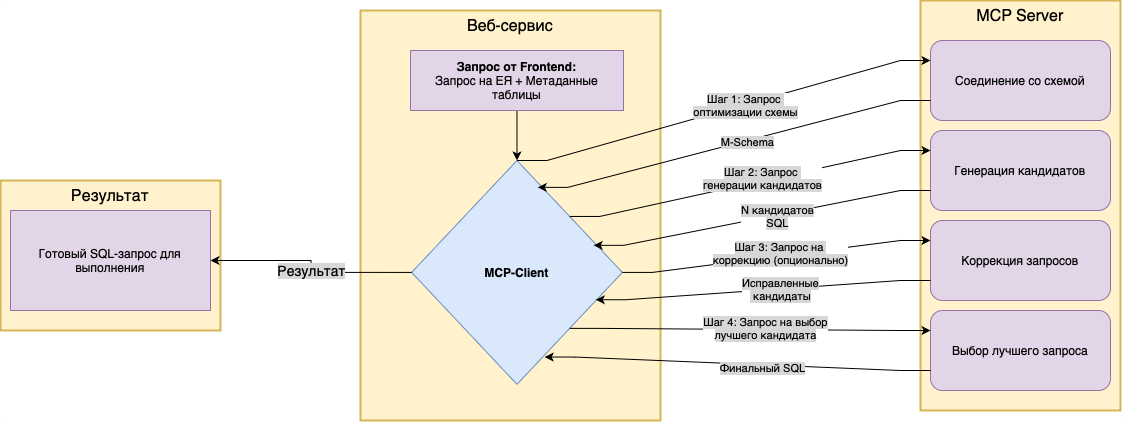
\includegraphics[width=1\textwidth]{created-diagrams/mcp-client-diagram.png}
	\caption{Модель взаимодействия MCP-клиента с MCP-сервером XiYan-SQL}
	\label{fig:mcp-client-flow}
\end{figure}

Данную модель можно описать следующими последовательно выполняющимися шагами:
\begin{compactenum}
	\item \textbf{Получение запроса}. MCP-клиент получает от основной логики бэкенда
	текст вопроса пользователя и метаданные целевой таблицы.
	\item \textbf{Связывание со схемой}. Клиент формирует и отправляет
	первый MCP-запрос к \textit{Модулю связывания схемы}. В ответ он получает
	оптимизированную схему данных (M-Schema).
	\item \textbf{Генерация кандидатов}. Используя полученную M-Schema,
	клиент параллельно обращается к нескольким \textit{Модулям генерации кандидатов},
	передавая им текст вопроса. В результате он получает несколько версий-кандидатов SQL-запроса.
	\item \textbf{Уточнение и коррекция (опционально)}. При необходимости клиент может
	передать полученных кандидатов \textit{Модулю уточнения} для автоматического
	исправления возможных ошибок. Этот шаг может быть итеративным.
	\item \textbf{Выбор лучшего кандидата}. Финальный набор кандидатов передается
	\textit{Модулю выбора}, который на основе своих внутренних метрик выбирает один,
	наиболее вероятный SQL-запрос.
	\item \textbf{Возврат результата}. MCP-клиент получает от \textit{Модуля выбора}
	финальный SQL-запрос и возвращает его основной логике бэкенда для последующего выполнения и
	отображения результата пользователю.
\end{compactenum}

Предложенная архитектура на основе MCP-клиента позволяет полностью абстрагировать
основное веб-приложение от сложности внутреннего устройства NLIDB-ядра. В следующей главе
будет описан процесс программной реализации прототипа веб-сервиса,
который использует данную архитектуру, где модуль MCP-клиента будет реализован с эмуляцией
вызовов к ядру XiYan-SQL.